% Search for all the places that say "PUT SOMETHING HERE".

\documentclass[11pt]{article}
\usepackage{amsmath,textcomp,amssymb,geometry,graphicx,enumerate,listings,graphicx}

\def\Name{Josiah Kim}  % Your name
\def\SID{948500821}  % Your student ID number (e.g. 938231937)
\def\Login{juk483} % Your login (e.g. pzm11)
\def\Homework{7} % Number of Homework
\def\Session{Spring 2021}


\title{CMPSC 465 -- Spring 2021 --- Solutions to Homework \Homework}
\author{\Name, SID \SID, \texttt{\Login}}
\markboth{CMPSC 465 --\Session\  Homework \Homework\ \Name}{CMPSC 465 --\Session\ Homework \Homework\ \Name, \texttt{\Login}}
\pagestyle{myheadings}

\newenvironment{qparts}{\begin{enumerate}[{(}a{)}]}{\end{enumerate}}
\def\endproofmark{$\Box$}
\newenvironment{proof}{\par{\bf Proof}:}{\endproofmark\smallskip}

\textheight=9in
\textwidth=6.5in
\topmargin=-.75in
\oddsidemargin=0.25in
\evensidemargin=0.25in


\begin{document}
\maketitle


\section*{1. Getting started}
\begin{qparts}
\item
I did not work in a group.
\item
I did not consult with any of my group members.
\item
I did not consult any non-class materials.
\end{qparts}



\newpage
\section*{2. Shortest Bitonic Paths}
\begin{qparts}
\item
\begin{lstlisting}

shortestPathsWithNegativeEdges(G, w, s):
	for all vertices u in V:
		dist(u) = infinity
 		prev(u) = null

	dist(s) = 0
 
	H = makequeue(V) using dist as the key

	while H is not empty:		
		u = deletemin(H)
		for all edges (u, v) in E:
			update((u, v))
			decreasekey(H, v)
		
		
\end{lstlisting}
This algorithm combines the update() method introduced in the Bellman-Ford Algorithm with Dijkstra's binary heap. 

Setting all vertices dist() to infinity and prev() to null will take a time of $O(|V|)$. The decreasekey() method will take $O(log|E|)$ time. Finally, the deletemin() method will take $O(log|E|)$ time. Therefore the entire while loop will take $O(|E|log|E|)$ time.

Total Runtime:$O(|V|)$ + $O(|E|log|E|)$ = $O(|V| + |E|log|E|)$

\item
\begin{lstlisting}
shortestPathBitonic(G, w, s):
	for all vertices u in V:
		dist(u) = infinity
 		prev(u) = null

	dist(s) = 0
 
	H = makequeue(V) using dist as the key

	while H is not empty:
		u = deletemin(H)
		for all edges (u, v) in E:
			if dist(u) > dist(v):
				insert(u) 
			update((u, v))
			decreasekey(H, v)

\end{lstlisting}
Taking advantage of the shortest-path algorithm for negative edge weights, I made a simple modification after the update() method. This conditional statement will inject back into the queue a vertex if not in increasing order. Therefore, the increasing edge weight assumtion can still be applied to this algorithm.

insert() has a time of $O(log|E|)$. This is negligible since the entire loop will take $O(|E|log|E|)$ time. Therefore, the runtime will stay the tsame: $O(|V| + |E|log|E|)$





\end{qparts}


\newpage
\section*{3. Dijkstra's on Negative}
\begin{qparts}


\item 

See hand-drawn graph below. 

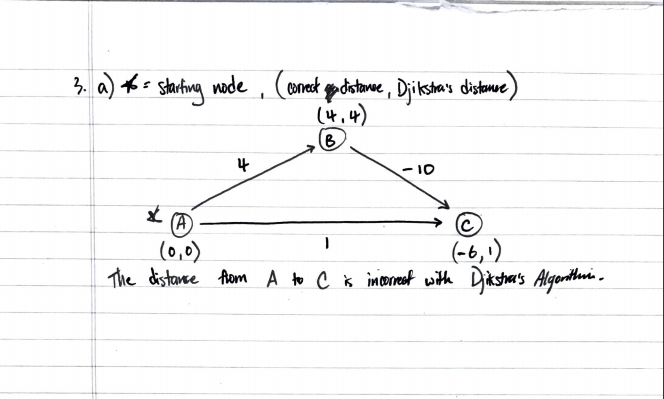
\includegraphics[scale=0.5]{hw7_q3a}

\item 
On the graph above, this assumption does not hold: "Also, because $x $ is in $R$, it must have removed from $H$ during a previous iteration and had all its outgoing edges updated." 

One the first iteration, $R=\{\}$ since $H = \{A, B, C\}$. Then, $R=\{A\}$. Then, $R=\{A, B\}$. At this point, $H = \{C\}$ which means that $B$ will not be visited again. Therefore, its outgoing edge (negative) to $C$ will not be found by the algorithm. This is because Dijkstra's Algorithm assumes that adding an edge will never make the path shorter, so it will no longer need to check a vertex again for a shorter path.  


\end{qparts}

\newpage
\section*{4.Greedy Choice}

We need to show that the third ingredient in the three key ingredients are satisfied to prove there exists an optimal greedy solution.\\

1. \\
We want to choose a portion of each item to put into the knapsack to maximize the weight. Each choice is an item to put in the knapsack. When a choice for an item is made, there leaves a subproblem to calculate how much of the item to put into the knapsack [0, 1]. \\

2. \\
Making the greedy choice in this problem would mean taking as much of an item as possible. Let $j$ be an item with the maximum value-per-pound $\frac{x_{i}}{w_{i}}$. There exists an optimal solution to put the most of $j$ in the knapsack as possible. \\ 
PROOF BY CONTRADICITON:
Say that there is a solution in which $j$ is not taken. In this situation, the item taken which is placed in the knapsack is $n$. We can assume that $n < j$ which means $\frac{x_{n}}{w_{n}} < \frac{x_{j}}{w_{j}}$ since no value is greater than the maximum amount, $j$. At this point, the knapsack is full. We then replace $n$ with $j$. This means that the knapsack weight increases by $\frac{x_{j}}{w_{j}}$ which is greater in weight than it was previously. This proves that there is a contradiction and the original solution is correct. \\

3. \\

\begin{lstlisting}
fractionalKnapsack(items):
	sort(v_j/w_j) in decreasing order
	for x in range 1 to n:
		take as much of item x as possible

\end{lstlisting}
 
If sorted in decreasing order by value-per-pound, this algorithm would take the most of the highest value-per-pound items until it reaches the weight limit. 


\newpage
\end{document}












